\documentclass[11pt]{beamer}
\usepackage[T1]{fontenc}
\usepackage[utf8]{inputenc}

\usepackage{pgf,pgfpages}
\usepackage{pgffor} % For loops

\usepackage{tikz}
\usetikzlibrary{arrows,shapes,backgrounds,calc}

\usepackage{graphicx}
\usepackage{colortbl}
\usepackage{units}

% \usepackage{calrsfs}
% \DeclareMathAlphabet{\pazocal}{OMS}{zplm}{m}{n}
% \usepackage{calligra}
\usepackage[cal=boondox,scaled=1.15]{mathalfa}
% \usepackage{bickham}
% \usepackage{boondox-cal}
% \usepackage{boondox-calo}
% \usepackage{dutchcal}

%% Beamer style >>>>>>>>>>>>>>>>>>>>>>>>>
\mode<presentation>
{
  \usetheme{PHD}
  \setbeamercovered{transparent}
  \setbeamertemplate{items}[square]
}

%\usefonttheme[onlymath]{serif}

\beamertemplatenavigationsymbolsempty

\defbeamertemplate{enumerate item}{mycircle}
{
  %\usebeamerfont*{item projected}%
  \usebeamercolor[bg]{item projected}%
  \begin{pgfpicture}{0ex}{0ex}{1.5ex}{0ex}
    \pgfcircle[fill]{\pgfpoint{-0.1pt}{.65ex}}{1.1ex}
    \pgfbox[center,base]{\color{PHDyellow}{\insertenumlabel}}
  \end{pgfpicture}%
}
[action]
{\setbeamerfont{item projected}{size=\scriptsize}}
\setbeamertemplate{enumerate item}[mycircle]

\setbeamertemplate{frametitle continuation}[from second][] % No automatic symbols I II II
%<<<<<<<<<<<<< beamer style

\title{Numerical Essays on Classical Keller-Segel Equations\vspace{-0.5em}}
\author[J.R. Rodr\'{\i}guez Galv\'an]{\em\structure{J. Rafael Rodr\'{\i}guez
  Galv\'an}\\\small Universidad de C\'adiz\vspace{-1.5em}}
\date{\Large{EDAN}\\\small Universidad de Sevilla. October 5, 2018}

% XeLaTeX font choosing
% \usepackage{fontspec}%{xltxtra} %fontspec}
% \setsansfont{Fontin Sans}
% \setsansfont{Lato}

% PDFLaTeX font choosing
\usepackage[default, scale=1.0]{lato}

\setbeameroption{hide notes} % Only slides
% \setbeameroption{show only notes} % Only notes
% \setbeameroption{show notes on second screen=right} % Both

% Different math fonts, see http://tug.org/pracjourn/2006-1/hartke/hartke.pdf
%\usepackage{eulervm}
%\usepackage{ccfonts, eulervm}
%\usepackage[math]{kurier}
%\usepackage[math]{anttor}
%\usepackage{pxfonts}
%\usepackage{mathpazo}
%\usepackage{mathpple}
%\usepackage[varg]{txfonts}
%\usepackage{arev}
%\usepackage{fourier}

% \usepackage{array, multirow, rotating} % booktabs: toprule, midrule...
\usepackage{array,booktabs,tabularx}

\newcommand{\heatProblem}{(Heat-Problem)\xspace}
\newcommand{\poissonProblem}{(Poisson-Problem)\xspace}

% % Video playing
% % Commands with two or more optional arguments
% % (see http://tex.stackexchange.com/questions/29973/more-than-one-optional-argument-for-newcommand)
% \usepackage{xparse} % From future LaTeX 3
% \DeclareDocumentCommand{\PlayVideoWithLabelAutostart}{%
%   O{0.5\linewidth} O{0.5\linewidth}  O{} m }{%
%   % #1: width of video box
%   % #2: height of video box
%   % #3: Label
%   % #4: Video file
%   \begin{BoxWithVerticalLabel}{#3}{#1}
%     \href{run:#4?autostart}{\rule{#1}{#2}}
%   \end{BoxWithVerticalLabel}}

% \DeclareDocumentCommand{\PlayVideoWithNoLabelAutostart}{%
%   O{0.5\linewidth} O{0.5\linewidth} m }{%
%   \href{run:#3?autostart}{\rule{#1}{#2}}}

% \DeclareDocumentCommand{\PlayVideoNOAutoStart}{%
%   O{0.5\linewidth} O{1.0} O{} m }{%
%   \href{run:#3}{\rule{#1}{#2}}}

% \DeclareDocumentCommand{\PlayVideoWithLabelNOAutostart}{%
%   O{0.5\linewidth} O{1.0} O{} m }{%
%   \begin{BoxWithVerticalLabel}{#3}{#1}
%     \href{run:#4}{\rule{#1}{#2}}
%   \end{BoxWithVerticalLabel}}

% \DeclareDocumentCommand{\PlayVideoWithLabel}{%
%   O{0.5\linewidth} O{1.0}  O{} m }{\PlayVideoWithLabelAutostart[#1][#2][#3]{#4}}

% % \DeclareDocumentCommand{\PlayVideoWithLabel}{%
% %   O{0.5\linewidth} O{1.0}  O{} m }{\PlayVideoWithLabelNOAutostart[#1][#2][#3]{#4}}

\usepackage{current-definitions}

\newtheorem{remark}{Remark}
\newtheorem{proposition}{Proposition}
%\newtheorem{theorem}{Theorem}

% Presentation goodies >>>>>>>>>>>>>>>>>>>>>>>>>>>>
\newcommand<>{\myframed}[1]{\alt#2{\tikz[phd] \node[box] {#1};}{{#1}}}
\newcommand<>{\myframedAlert}[1]{\alt#2{\tikz[phdB] \node[boxB] {\color{black}#1};}{{#1}}}
\newcommand<>{\framedmath}[1]{%
\alt#2{\tikz[phd] \node[box] {\ensuremath{#1}};}{\ensuremath{#1}}}
\newcommand{\framedB}[1]{\tikz[phd] \node[boxB] {#1};}
\newcommand{\framedmathB}[1]{\framedB{\ensuremath{\displaystyle{#1}}}}
\newcommand{\ver}[1]{\footnote{See #1}}
\newcommand{\cita}[1]{{\color{PHDgray}\cite{#1}}}
\newcommand\cellalert[2]{\only<#1>{\cellcolor{PHDyellow}}\alt<#1>{\textbf{#2}}{#2}}
\newcommand{\soften}[1]{{\color{PHDgray}#1}}
\newcommand{\rowalert}[7]{%
    \cellalert{#1}{#2} & \cellalert{#1}{#3} &
    \cellalert{#1}{#4} & \cellalert{#1}{#5} &
    \cellalert{#1}{#6} & \cellalert{#1}{#7}}

\newcommand{\kk}{\Delta t}
\newcommand{\Tmax}{\ensuremath{T_{\mbox{max}}}}

% \usepackage{wasysym}
% \newcommand{\good}{{\color{PHDgreen}$\CIRCLE$}} %\blacksmiley
% \newcommand{\bad}{{\color{PHDred}$\CIRCLE$}}
\usepackage{pifont, fontawesome}
\newcommand{\good}{{\color{PHDgreen}\ding{52}}}
\newcommand{\bad}{{\color{PHDred}\ding{56}}}
\newcommand{\exclamation}{{\large\color{PHDred}{\textbf{\itshape !}}}}
\newcommand{\question}{{\large\color{PHDred}{\textbf{\itshape ?}}}}
\newcommand\colorUnderLine[2][PHDyellow]{\color{#1}\underline{{\color{black}#2}}\color{black}\xspace}
\newcommand\gris[1]{{\color{PHDgray}#1}}
\newcommand\amarillo[1]{{\color{PHDyellow}#1}}
\newcommand\tiragris[1]{{\par\hfill\small\gris{#1}}}
\newcommand\point{\alert{\faHandORight}\xspace}
%<<<<<<<<<<<<<<<

\setcounter{tocdepth}{1}


%
% Bibliography
%
%\usepackage{natbib}

% To list each bibliographic entry in a line
\setbeamertemplate{bibliography entry title}{}
\setbeamertemplate{bibliography entry location}{}
\setbeamertemplate{bibliography entry note}{}

% ... end of preamble.

\AtBeginSection{\frame{\sectionpage}}

\renewcommand{\vv}{v}
\renewcommand{\VV}{V}

%======================================================================
\begin{document}
%======================================================================

% Tikz style and beamer template ------->>>
\tikzstyle{every picture}+=[remember picture]
\tikzstyle{na} = [baseline=-.5ex]
\tikzstyle{phd} = [baseline=-.6ex,
  box/.style={rectangle, draw=PHDblueC, thick, fill=PHDblueA,
    align=center, rounded corners, minimum height=1.6em},
  boxB/.style={rectangle, draw=PHDredA, thick, fill=PHDblueA,
    align=center, rounded corners, minimum height=1.6em}]
\tikzstyle{phdB} = [baseline=-.7ex,
  box/.style={rectangle, draw=PHDblueC, thick, fill=PHDblueA,
    align=center, rounded corners, minimum height=1.6em},
  boxB/.style={rectangle, draw=PHDredA, thick, fill=PHDblueA,
    align=center, rounded corners, minimum height=1.6em}]
\tikzstyle{myarrow} = [->,>=latex, PHDredA, shorten >=4pt,
  opacity=.6, line width=0.6mm]
\tikzstyle{myarrow2} = [->,>=latex, PHDblueC, shorten >=4pt, opacity=.2, line width=0.4mm]
\tikzstyle{myarrow3} = [
     opacity=.7,
%    >=triangle 60,              % Nice arrows; your taste may be different
    node distance=6mm and 60mm, % Global setup of box spacing
    every join/.style={norm},   % Default linetype for connecting
                                % boxes
    line width=0.6mm,
    PHDredA,
    ->
    ]
\setbeamertemplate{background}
 {
\includegraphics[width=\paperwidth,height=\paperheight]{frontpage_bg}}
\setbeamertemplate{footline}[default]
% <<<-------


% Write custom titlepage ------->>>
\begin{frame}
  \titlepage
  \vspace{5cm}
\end{frame}

% Set the background for the rest of the slides.
\setbeamertemplate{background}{}
 % {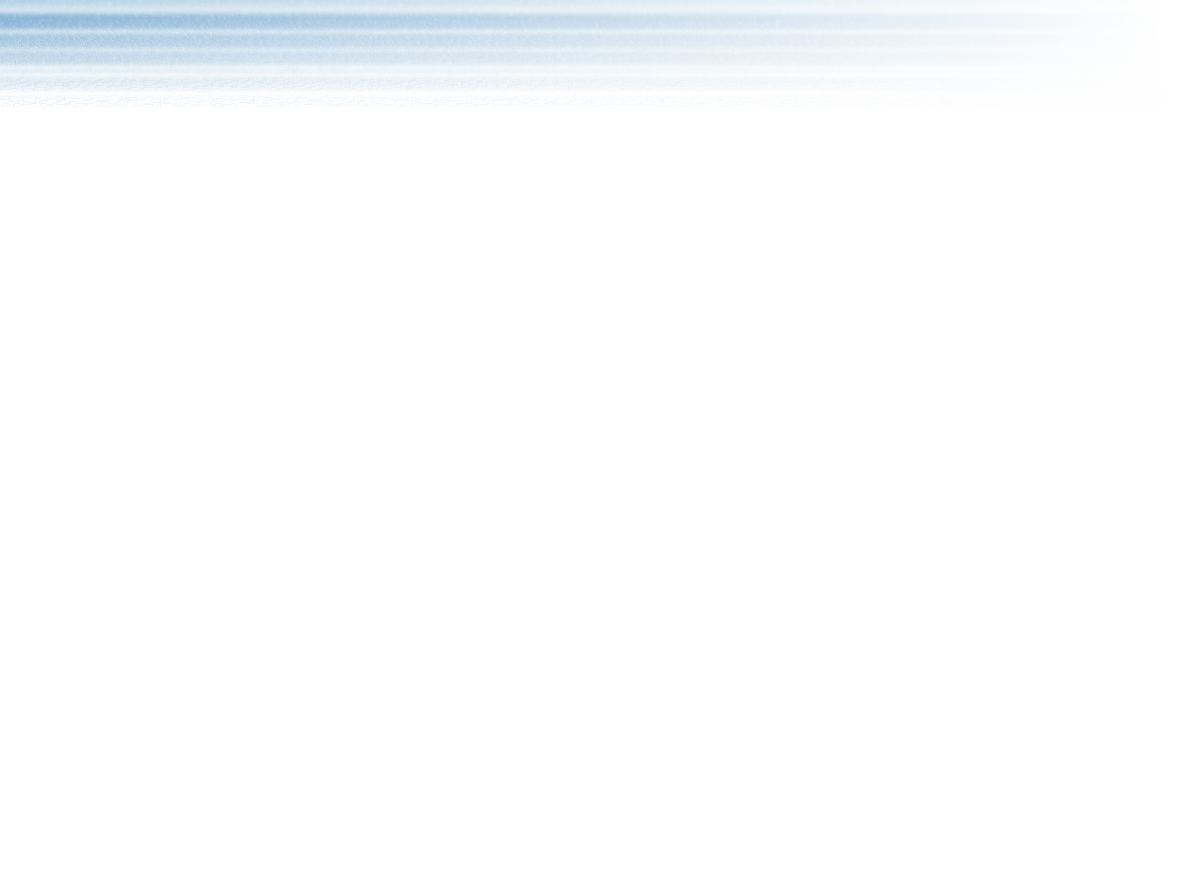
\includegraphics[width=\paperwidth,height=\paperheight]{slide_bg}}


% Write all of the slides..........

\begin{frame}{Outline}
  \tableofcontents
\end{frame}

% Start inserting infoline at the end
\setbeamertemplate{footline}[PHDtheme]
% <<<-------

\newcommand{\imgdir}{Undefined, use renewcommand!}

%============================================================================
\section{Definitions and Some Analysis}
%============================================================================

%=====================================================================
\begin{frame}{Chemotaxis}
%---------------------------------------------------------------------
  \begin{itemize}\itemsep1em
  \item Movement of \structure{biological cells} in response
    to \structure{chemical signals}
  \item  \alert{General formulation} (\structure{Keller--Segel} 1970')~\cite{winkler_bellomo_toward_2015}
    \par\bigskip
    \begin{quotation}
    Find \structure{$u$}, \structure{$v$} (\textit{density of cells} and
    \textit{chemical-signal}) such that:
  \begin{equation*}\def\arraystretch{1.2}
    \label{K-S}
    \left\{
      \begin{array}{ll@{}}
        u_t= \div\Big( D_u(u,v)\*\grad u - \chi(u,v) \* u \* \nabla v\Big) + H(u,v), \\
        v_t= D_v(u,v)\*\Delta v + K(u,v)
      \end{array}\right.
  \end{equation*}
\end{quotation}
\item Many variants\footnote{See e.g.~\cite{horstmann_2003}
    for a review}  depending on (likely nonlinear) terms...
  \par\smallskip
  \begin{itemize}\itemsep0.66em
  \item Source terms: $H(u,v)$, $K(u,v)$
  \item Diffusion of cells and chemoattractant:  $D_u(u,v)$, $D_v(u,v)$
  \end{itemize}
\end{itemize}

\end{frame}

%=====================================================================
\begin{frame}{The Classical Keller-Segel System}
%---------------------------------------------------------------------
  We focus on the \textit{classical system}
    in $\Omega\times(0,T)\subset\mathbb{R}^{n+1}$:
    \begin{quotation}
  \begin{equation*}\def\arraystretch{1.2}
    \label{K-S}
    \left\{
      \begin{array}{ll@{}}
        u_t= \kA\Delta u - \alert{\kB\nabla\cdot( u\nabla v)}, &  \quad {\color{gray}x\in\Omega,\, t>0,}\\
        v_t= \kC\Delta v - \kD v + \kE u, &  \quad {\color{gray}x\in\Omega,\, t>0.}
      \end{array}\right.
  \end{equation*}
\end{quotation}
  \begin{itemize}\itemsep0.66em
  \item Parameters $\alpha_i>0$. In particular $\alpha_1>0$
    $\Rightarrow$ \structure{chemoattractant} model
  \item \alert{Nolinear chemotaxis term}! {\color{gray}Hyperbolic effects expected if $\alpha_1\!\gg$}
  \item Boundary conditions
    $$
    \frac{\partial u}{\partial \nu}=\frac{\partial v}{\partial \nu}=0, {\color{gray}\quad x\in\partial\Omega,\, t>0.}
    $$
  \item Initial conditions (important \structure{rule in long-time} behaviour):
    $$ u(x,0)=u_0(x), \quad v(x,0)=v_0(x), \qquad {\color{gray}x\in\Omega.}$$
\end{itemize}

\end{frame}
%=====================================================================



%=====================================================================
\begin{frame}{Local Existence, Positivity and Blow-up}
%---------------------------------------------------------------------
  A general result\footnote{%
    \color{gray} This result is also valid for more general
    Keller-Segel equations see
    e.g.~\cite{winkler_bellomo_toward_2015}, Lemma~3.1}:
  \medskip
  \begin{itemize}\itemsep1em
  \item If \structure{$u_0\in C^0(\overline\Omega)$},\enspace
    \structure{$v_0\in W^{1,q}(\Omega)$} \small non-negative \gris{($q>n=\mbox{space
      dim.}$)}
  \item Then \enspace \llaveizq{$\structure{\exists \Tmax} \in(0,+\infty]$ and\\[0.9ex]
    $\alert{\exists!u, v}\in C^0\big(\overline\Omega\times
      (0,\Tmax)\big)$} \quad such that\footnote{%
      \color{gray} In fact, also
      $u, v\in C^{2,1}\big(\overline\Omega\times [0,\Tmax)\big)$
      $v\in L^\infty_{\mbox{loc}}([0,\Tmax); W^{1,q}(\Omega))$}
    % \begin{align*% }
    %   \alert{u, v\in C^0\big(\overline\Omega\times (0,\Tmax)\big)}
    % \end{align*}
    % such that
    \medskip
    \begin{itemize}\itemsep0.66em
    \item $(u,v)$ \alert{solves classical} \alert{Keller-Segel} equations in $\Omega\times (0,\Tmax)$
    \item \alert{$u,v\ge 0$} (positivity of solution)
    \item If $\structure{\Tmax<+\infty}$ $\Rightarrow$
      $\alert{\norm[L^\infty(\Omega)]{u}} +
      \alert{\norm[W^{1,q}(\Omega)]{v}}\to\infty$ as $t\nearrow\Tmax$
  \end{itemize}
\item \small We say that \structure{$u$ blows up} in $\Tmax$ if
      $\alert{\norm[L^\infty(\Omega)]{u}}\to\infty$ as $t\nearrow\Tmax$.
  \end{itemize}
\end{frame}
%=====================================================================

%=====================================================================
\begin{frame}{Other Properties}
%---------------------------------------------------------------------
  \begin{itemize}
  \item \alert{Mass conservation}: If $u$ is a regular enough solution
    in $\Omega\times(0,T)$,
    $$
    \int_\Omega u(\cdot,t) = \int_\Omega u_0 \quad \forall t\in(0,T).
    $$
  \item \alert{Energy dissipation}:
    $$
    \structure{\frac{d}{dt}\E\big(u(\cdot,t),v(\cdot,t)\big)
    =
    -\D\big(u(\cdot,t),v(\cdot,t)\big)} \quad \forall t\in(0,T),$$
    \small
    with
    \begin{align*}
     \E(u,v)&=\frac12 \int_\Omega |\grad v|^2 + \int_\Omega v^2 - \int_\Omega u\*v + \int_\Omega u\*\ln u,\\
     \D(u,v)&=\int_\Omega v_t^2+ \int_\Omega \left| \frac{\grad u}{\sqrt u} - \sqrt u \grad v \right|^2.
    \end{align*}
    \point \textit{Crucial role in theoretical results (global existence, blow-up...)}
  \end{itemize}
\end{frame}
%=====================================================================

%=====================================================================
\begin{frame}{Theorem (Global Existence and Boundedness)}
%---------------------------------------------------------------------

  \begin{scriptsize}
  \begin{itemize}
  \item  Assume $u_0\in C^0(\overline\Omega)$, \enspace
    $v_0\in \bigcup_{q>n} W^{1,q}(\Omega)$,
  \item  Let
    $(u,v)$ maximal solution of classical K-S.
  \end{itemize}
\end{scriptsize}
  \textbf{Then}
  \begin{itemize}\itemsep1em
  \item If \alert{$n=1$} or \alert{$n=2$} \big(with \structure{$\int_\Omega u_0<4\pi$} for $n=2$\big)%
    \footnote{\gris{It is enough $\int_\Omega u_0 <8\pi$ if $\Omega$ is a disc and $(u_0,v_0)$ radially symmetric}}
    \par\medskip
    \quad $\Rightarrow$\enspace $(u,v)$ \emph{exists globally}  in time and is bounded, i.e.
    $$
    \structure{
      \norm[L^\infty(\Omega)]{u(\cdot,t)}
      +\norm[L^\infty(\Omega)]{v(\cdot,t)} \le C} \quad \forall t>0.
  $$
\item If \alert{$n\ge 3$}: $\exists \varepsilon,\lambda >0$ such that
  \begin{small}\vspace{-0.5em}
    $$
    \mbox{if}\quad
    \norm[L^{n/2}(\Omega)]{u_0}<\varepsilon, \quad
    \norm[W^{1,n}(\Omega)]{u_0}<\varepsilon,
    $$
  \end{small}
    \quad$\Rightarrow$ $(u,v)$ \emph{exists globally} in time and satisfies
    $$
    \structure{    \norm[L^\infty(\Omega)]{u(\cdot,t)-\overline{u_0}}
      + \norm[L^\infty(\Omega)]{v(\cdot,t)-\overline{v_0}} \le C e^{-\lambda t}}
      \quad\forall t>0.
    $$
  \end{itemize}
  \vfill
\end{frame}
%=====================================================================


%============================================================================
\section{Time Schemes}
%============================================================================

%=====================================================================
\begin{frame}{Time Discretization}
%---------------------------------------------------------------------
  \begin{small}
  Let
  \begin{itemize}
  \item $0=t_0<t_1<\cdots<t_N=T$
  \item $k=\tmm-\tm$, \quad
    $\um\approx u(\tm)$, \quad $\forall m=0,...,N$
  \end{itemize}
\end{small}
  \smallskip
  \begin{block}{\textbf{\color{white}{Euler Time Scheme Family}}}
    \vspace*{-0.5em}
    \begin{large}
  \begin{align*}
    (1/k)\umm &- \Delta\umm + \div(u^{\alert{m+s_1}}\grad v^{\alert{m+s_2}} ) = (1/k)\um
    \\[0.7em]
    (1/k)\vmm &- \Delta\vmm + v^{\alert{m+s_3}} - u^{\alert{m+s_4}} = (1/k)\vm
  \end{align*}
\end{large}
  % where $r_1$, $r_2$, $r_3$, $r_4$ $\in\{0,1\}$,
  where ${S}=(s_1,s_2,s_3,s_4)\in\{0,1\}^4$.
\end{block}
\begin{itemize}\itemsep0.5em
\item All of them are implicit; the scheme $S=(1,1,1,1)$ is fully implicit
\item We are interested \structure{discrete energy} laws for
  \structure{linear} and \structure{uncoupled} schemes
%   \smallskip
%   \begin{center}
%   \begin{small}
%   \begin{tabular}[c]{llll}
%     \toprule
%   $(0,0,0,0)$& $(0,0,0,1)$& $(0,0,1,0)$& $(0,0,1,1)$ \\ \hline
%   $(1,0,0,0)$& $(1,0,0,1)$& $(1,0,1,0)$& $(1,0,1,1)$ \\
%     \bottomrule
%   \end{tabular}
% \end{small}
% \end{center}
\end{itemize}
\end{frame}

%=====================================================================

%=====================================================================
\begin{frame}{Proposition (Discrete Energy Laws)}
%---------------------------------------------------------------------
  \begin{small}
    If $\big\{(\um,\vm)\big\}_{m=0}^N$ sufficiently regular
    solution of scheme $S=(s_1,s_2,s_3,s_4)$:
\end{small}
\bigskip
  \begin{equation*}
    \alert{\ddt\Emm_S \le - \Dmm_S - \Nmm_S + \Mmm_S} \gris{\small,\quad \forall m=0,...,N-1},
  \end{equation*}
\medskip
  \small
  where
  \begin{align*}
    \Emm_S &= \E(\umm,\vmm), \\[0.4em]
    \Dmm_S &= \int_\Omega \big(\ddt \vmm\big)^2
           + \int_\Omega \left| \frac{\grad \umm}{\sqrt \umm} - \sqrt \umm \grad \vmm \right|^2, \\[0.4em]
    \Nmm_S &= \frac k 2 \int_\Omega \big(\dt\grad\vmm\big)^2 + N_{1,S} + N_{2,S}+ N_{3,S}+ N_{4,S}, \\[0.4em]
    \Mmm_S &= M_{1,S} + M_{2,S} + M_{3,S} +M_{4,S}.
  \end{align*}
  \medskip
  \begin{small}
    Here:
    \vspace*{-1em}
    \begin{itemize}
    \item $\ddt(\wm)=(\wmm-\wm)/k$,
\item
  \structure{$N_{i,S}$, $M_{i,S}$ $\ge 0$} (numerical dissipation and sources),
  \structure{$N_{i,S},M_{i,S} \to 0$} as $k\to 0$.
\end{itemize}
\end{small}
\end{frame}
%=====================================================================

%=====================================================================
\begin{frame}{Proof}
%---------------------------------------------------------------------
  \structure{Similar to continuous Energy Law}, using following
  properties:
  \bigskip
  \begin{itemize}\itemsep1em
  \item $\displaystyle \ddt(\wmm)\wmm=\frac12 \ddt(\wmm)^2 + \frac k2 (\ddt \wmm)^2$
    \enspace \gris{$\forall m \ge 0$,}
  \item $\displaystyle \ddt(\umm\cdot\vmm) = \um\dt\vmm + \vmm\dt\umm$
    \enspace \gris{$\forall m \ge 0$,}
  \item $\displaystyle b\, \big(\!\log a - \log b \big) \le a-b$
    \enspace \gris{$\forall a,b>0$,}
  \item $\displaystyle \int_\Omega \ddt\umm = 0$
    \enspace\gris{$\forall m\ge 0$} (\alert{discrete conservation of mass}).
  \end{itemize}
  \qed
\end{frame}
%=====================================================================

%=====================================================================
\begin{frame}{Optimal \structure{(?)} Time Scheme: $S=(1,1,1,0)$}
%---------------------------------------------------------------------
  ~\vspace*{-1em}
  \begin{align*}
    (1/k)\umm &- \Delta\umm + \div(u^{\alert{m+1}}\grad v^{\alert{m+1}} ) = (1/k)\um,
    \\[0.7em]
    (1/k)\vmm &- \Delta\vmm + v^{\alert{m+1}} - u^{\alert{m}} = (1/k)\vm.
  \end{align*}
  \small\vspace*{-1.3em}
  \begin{itemize}\itemsep0.4em
  \item Uncoupled (first compute $\vmm$, then $\umm$)
  \item $N_{i,S}=0$\gris{, $i=1,...,4$} $\Rightarrow$
  $\Nmm_S = \frac k 2 \int_\Omega \big(\dt\grad\vmm\big)^2$ \alert{minimizes dissipation}.
  \item $M_{i,S}=0$\gris{, $i=1,...,4$} $\Rightarrow$
  $\Mmm_S = 0$ \alert{minimizes numerical sources}.
  \end{itemize}
  \medskip
  Energy law:
  \begin{equation*}
    \alert{\ddt\Emm_S \le - \Dmm_S - \Nmm_S \le 0}
    \ \Rightarrow \ \alert{\Emm_S\searrow 0}.
  \end{equation*}
  Conjectures:
  \begin{align*}
    \ddt\Emm_S &= \min_{S'\in\{0,1\}^4} \ddt\Emm_{S'}\ \alert{\mathbf{???}}\quad
    \Emm_S = \min_{S'\in\{0,1\}^4} \Emm_{S'} \hfill\ \alert{\mathbf{???}}
    \\
    \norm[L^\infty(\Omega)]{u^{m}_S} &\le \norm[L^\infty(\Omega)]{u^m_{S'}}
                                       \quad \forall S'\in\{0,1\}^4 \ \alert{\mathbf{???}}
  \end{align*}
\end{frame}
%=====================================================================

%=====================================================================
\begin{frame}{Do Not Leave the Simulations for The End!}
%---------------------------------------------------------------------
  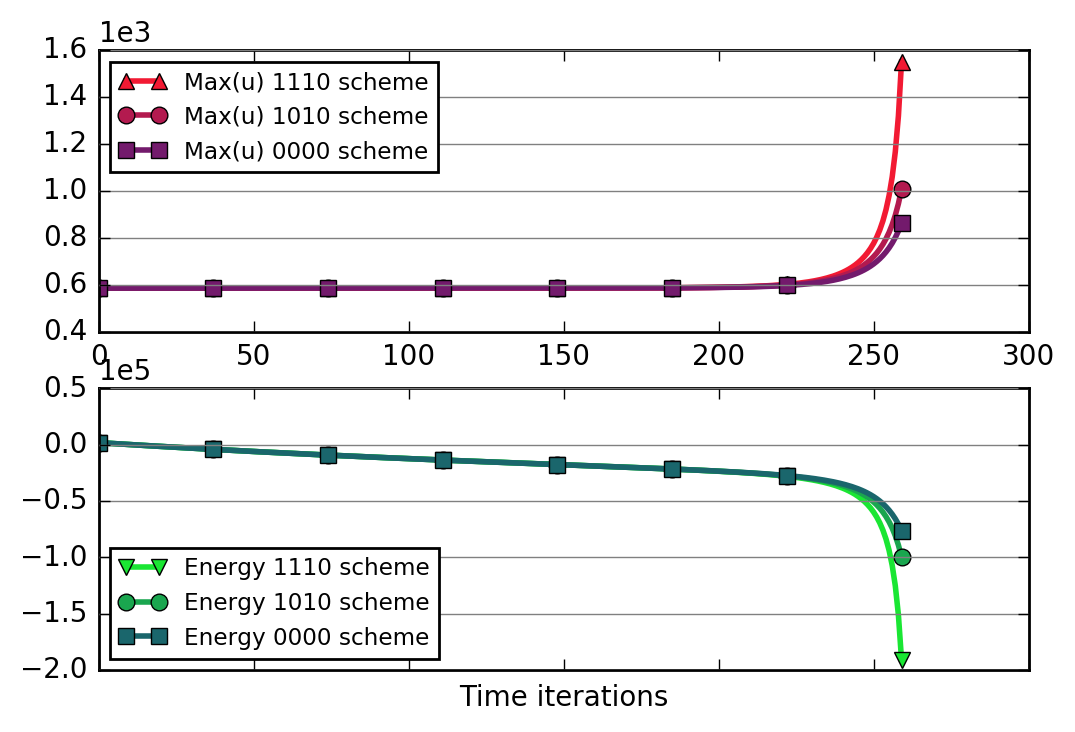
\includegraphics[width=0.98\linewidth]{img/energy-L2}
\end{frame}
%=====================================================================

%============================================================================
\section{Space Discretization}
%============================================================================

%=====================================================================
\begin{frame}{FEM Space Discretization}
%---------------------------------------------------------------------
  \begin{itemize}\itemsep1em
  \item For any Euler scheme $S\in\{0,1\}^4$,
    \begin{flushright}
      we approximate $(\um,\vm)$ at each time $\tm$ by means of \textbf{FEM}
    \end{flushright}
  \item All right (apparently)...\par\smallskip \hfill e.g. let us
    reproduce the following \structure{\textbf{numerical
      test}~\cite{farina_explicit_2015}}:
    \par\bigskip
    \begin{scriptsize}\color{darkgray}
      \begin{itemize}\itemsep0.5em
      \item $\Omega=[-2,2]^2\subset\mathbb{R}^2$
      $(\alpha_0,\alpha_1,\alpha_2,\alpha_3,\alpha_4) = (1,0.2,1,0.1,1)$
    \item $u_0= 1.15 e^{-(x^2+y^2)}(4-x^2)^2 (4-y^2)^2$ \alert{($\int_\Omega u_0 > \pi/4$, blow-up!)}
      $v_0=0.55 e^{-(x^2+y^2)} (4-x^2)^2 (4-y^2)^2$
    \item Time discretization: Euler scheme $S=(0,0,0,0)$
    \item Discretization: P1-Lagrange $\alert{200\times 200}$ mesh
      ($h\sim 10^{-2}$), $k=10^{-4}$
    \end{itemize}
    \end{scriptsize}

  \end{itemize}
\end{frame}
%=====================================================================


%=====================================================================
\begin{frame}[allowframebreaks]{Blow-up Test (plotting $u$)}
%---------------------------------------------------------------------
  \foreach \i in {1,...,16,20} {
    \begin{center}
      \includegraphics[width=0.85\linewidth]{img/viglialoro/ks_viglialoro_\i}%
    \end{center}
    \framebreak
    }
\end{frame}

%=====================================================================
\begin{frame}{Maximum Density of \alert{Cells} Over Time}
%---------------------------------------------------------------------
  \begin{center}
  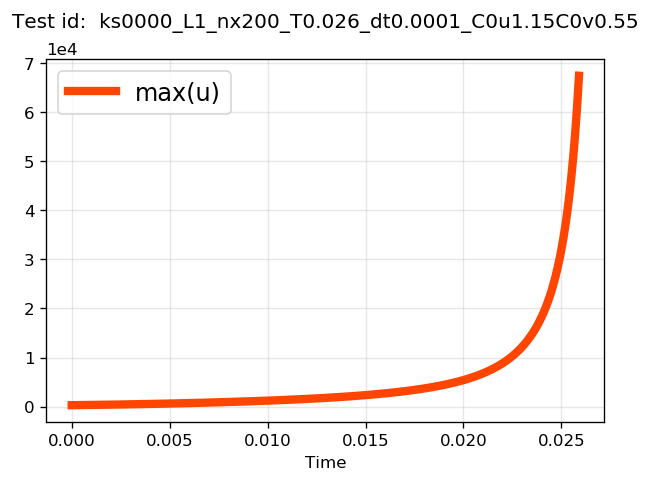
\includegraphics[width=0.8\linewidth]{img/viglialoro/viglialoro_max_u}%
\end{center}
\end{frame}

%=====================================================================
\begin{frame}{Maximum \structure{Chemical Agent} Over Time}
%---------------------------------------------------------------------
  \begin{center}
    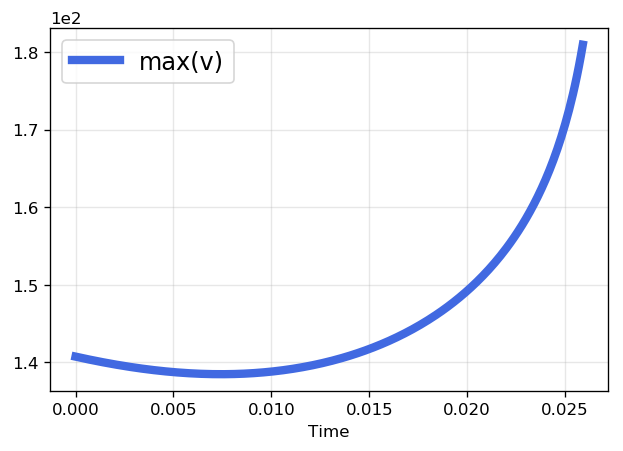
\includegraphics[width=0.8\linewidth]{img/viglialoro/viglialoro_max_v}%
    \\
    \textbf{\Large \textit{Positivity} of $u$ is broken due to FE
      approximation!}
    \end{center}
\end{frame}

%=====================================================================
\begin{frame}{\alert{Minimum} \alert{Cells} Over Time}
%---------------------------------------------------------------------
  \begin{center}
    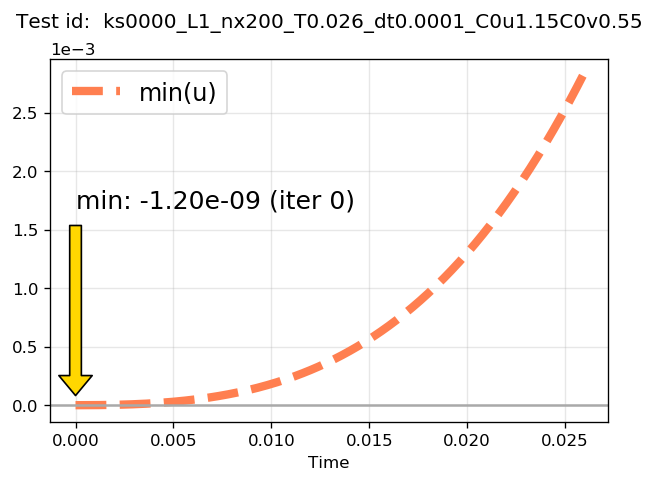
\includegraphics[width=0.8\linewidth]{img/viglialoro/viglialoro_min_u}%
    \\
    \textbf{\large \textit{Positivity} of $u$ is broken due to FE
      approximation!}
    \end{center}
\end{frame}

%=====================================================================
\begin{frame}[allowframebreaks]{\alert{Minimum} \alert{Cells} in a \structure{Coarser Grid} (nx=30)}
%---------------------------------------------------------------------
  \begin{center}
  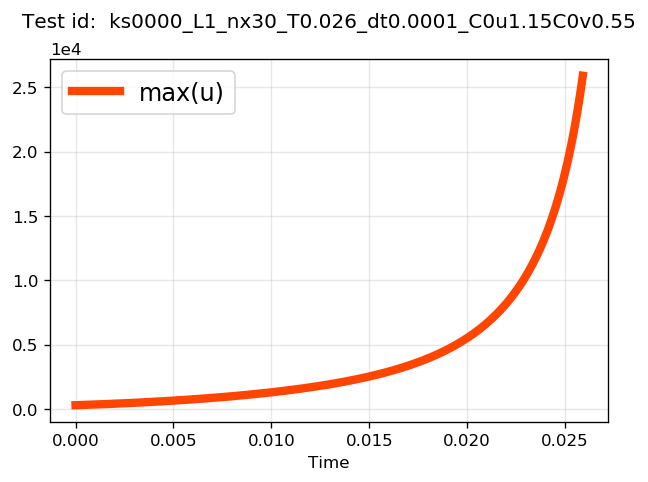
\includegraphics[width=0.8\linewidth]{img/viglialoro/viglialoro_max_u_nx30}%
  \\
  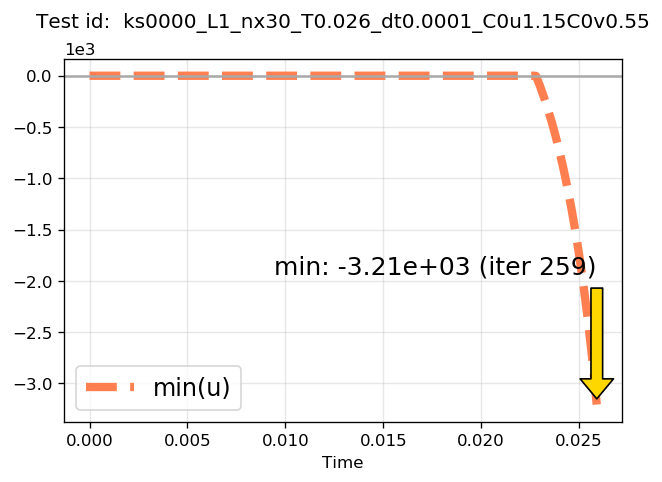
\includegraphics[width=0.8\linewidth]{img/viglialoro/viglialoro_min_u_nx30}
  \\
  \textbf{\large  \textit{Positivity} of $u$ is broken near blow-up time}
\end{center}
\end{frame}

%=====================================================================
\begin{frame}{... also positivity lost at initial time!}
%---------------------------------------------------------------------
  \begin{center}
    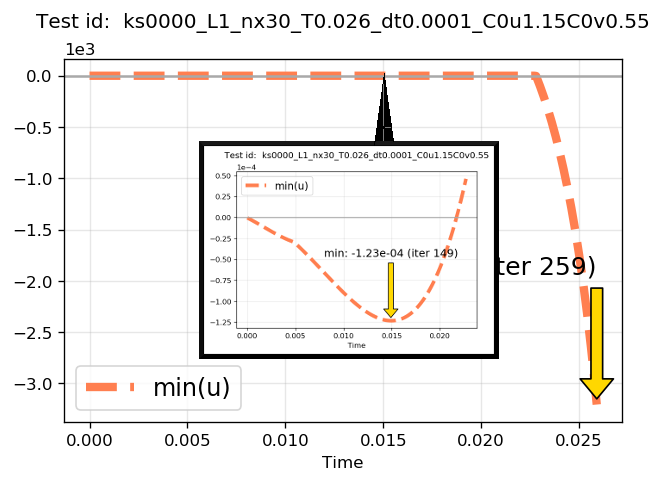
\includegraphics[width=0.9\linewidth]{img/viglialoro/viglialoro_min_u_nx30-zoom}%
    \end{center}
\end{frame}

%=====================================================================
\begin{frame}{Other Euler Schemes do Not Improve Positivity}
%---------------------------------------------------------------------
  \begin{itemize}
  \item E.g. similar (slightly better) results are obtained
    for \alert{$S=(1,1,1,0)$ }\vfill
  \begin{center}
    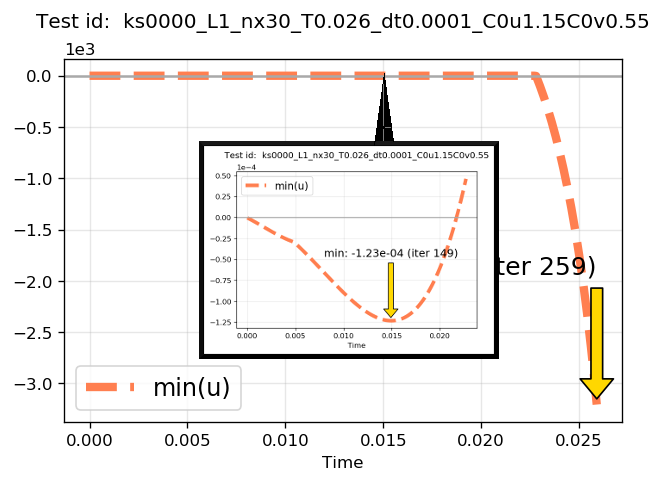
\includegraphics[width=0.6\linewidth]{img/viglialoro/viglialoro_min_u_nx30-zoom}%
    \end{center}
  \item Let us check other \textbf{FE space approximations}...
  \end{itemize}
\end{frame}

%=====================================================================

%=====================================================================
\begin{frame}{FreeFem++ and LibMesh}
%---------------------------------------------------------------------
  \begin{itemize}\itemsep0.6em

  \item We used the excellent well-known \textbf{\alert{FreeFem++}}
    suite for $P_1$ or $P_2$ \structure{\textbf{rapid}} \&
    \structure{\textbf{efficient}} software development!
  \item And also the \emph{C++ FE library} ``\textbf{\alert{LibMesh}}''
    \begin{itemize}\itemsep0.5em
    \item  \textbf{Open source}, built over other high-quality
      libraries
  \item \textbf{Parallel}, using \textbf{\textit{PETSc}} or
    \textit{Trilinos} as linear algebra bakends
  \item 1D, 2D, 3D \textbf{generic programming}
  \item \textbf{Variety of Finite Element polynomial families}:
    \begin{itemize}
    \item Classical $P_k$-Lagrange
    \item Hierarchical high-order Lobatto (order greater than 20)
    \item Bernstein positive polynomials
    \item Discontinuous $P_k$
    \item ...
    \end{itemize}
  \item Element \textbf{geometries}: triangles, squares, tetrahedrons
  \end{itemize}
\item {\footnotesize Other possibilities: \structure{DEAL.ii},
    \structure{DUNE}, \structure{MFEM}, \structure{FEMPAR}
    (S. Badia et al)...}
\item \alert{Cons} and \alert{pros}: When is the \textbf{price of high
    performance} worth?
  \end{itemize}
\end{frame}
%=====================================================================

%=====================================================================
\begin{frame}{Lobatto Polynomials in $I=(-1,1)$}
%---------------------------------------------------------------------
  ~\vspace*{-1em}
  \small
  \begin{align*}
    l_0(x)&=\frac{1-x}2
    \\
    l_1(x)&=\frac{1+x}2
    \\
    l_p(x)&=\frac1{\norm[2]{L_{p-1}}}\int_{-1}^x L_{p-1}(\xi)\,d\xi,
            \enspace p\ge 2, \ L_p=\mbox{\footnotesize Legendre polynomials}
  \end{align*}
  ~\vspace*{-0.3em}
  \begin{itemize}
  \item \alert{Hierarchical basis} in $\mathbb{P}_p$ ($\Rightarrow$ $p$--adaptivity)
  \item Suitable for continuous global basis in FE
  \item Ortogonality of $l'_p(x)$ in $L^2(-1,1)$
  \item \alert{Optimal condition number} of stiffness matrix as $p\to+\infty$
  \end{itemize}
  \begin{center}
  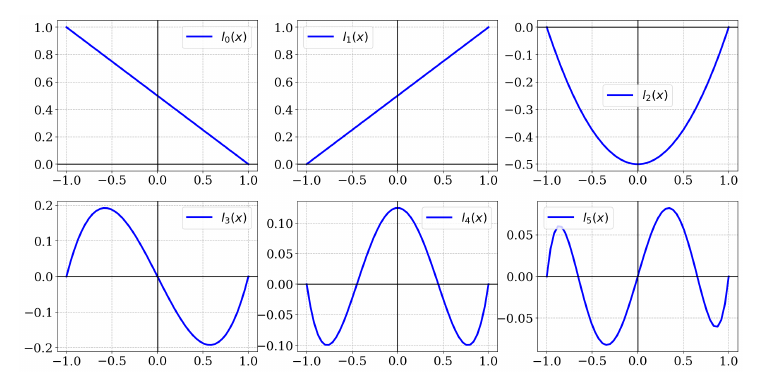
\includegraphics[width=0.47\linewidth]{img/lobatto-basis}
\end{center}
\end{frame}
%=====================================================================


%=====================================================================
\begin{frame}{Bernstein Polynomials in $I=(0,1)$}
%---------------------------------------------------------------------)
  \small
  \begin{align*}
    B_i^p(x)=\begin{pmatrix}p\\i\end{pmatrix}x^i(1-x)^{m-1},
    \quad p\ge 0,\ i=0,...,p
  \end{align*}
  \begin{itemize}
  \item (Not hierarchical) \alert{basis} in $\mathbb{P}_p$
  \item Suitable for continuous FE global basis
  \item Simmetry
  \item \alert{Positivity}: $B_i^p(x)\ge 0$ $\forall i,p$
  \end{itemize}
  \begin{center}
  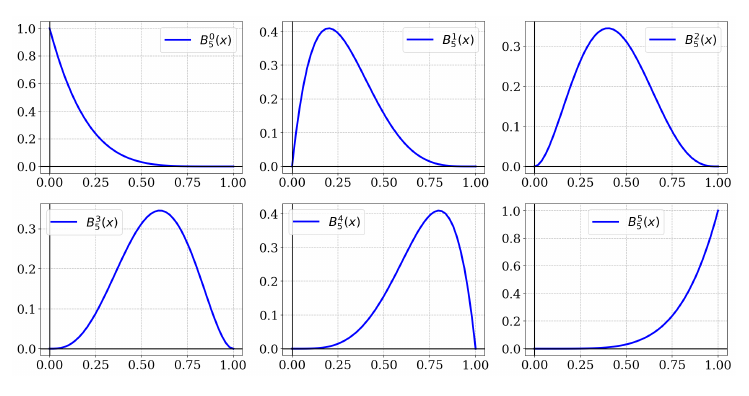
\includegraphics[width=0.47\linewidth]{img/bernstein-basis}
\end{center}
\end{frame}
%=====================================================================

%=====================================================================
\begin{frame}{Hierarchical (Lobatto) \alert{Order 8} 2D FE Test}
%---------------------------------------------------------------------
  \begin{itemize}\itemsep0.5em
  \item We run the following test (using \alert{LibMesh} in \structure{\texttt{valle.uca.es}}):
  \begin{itemize}\itemsep0.2em
  \item Time scheme: $S=(1,0,1,0)$, $\Tmax=0.026$, $k=0.001$
  \item Space scheme: Lobatto order 8 polynomial in mesh $30\times 30$
  \end{itemize}
\item \alert{CPU time} for 1, 2, 4,... , 32 processors (7m50s\dots 0m48s):\vspace*{-0.1em}
  \begin{center}
    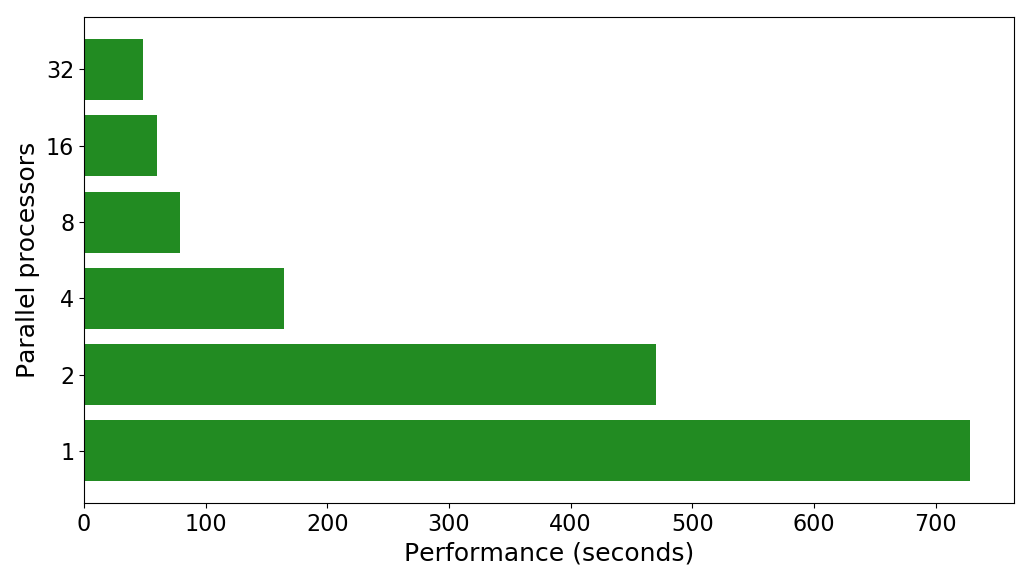
\includegraphics[width=0.98\linewidth]{img/cpu_times}%
  \end{center}
\end{itemize}
\vfill~
\end{frame}
%==================================================================


%=====================================================================
\begin{frame}{Results (of Former Test) Are Correct }
%---------------------------------------------------------------------
  \begin{tabular}{cc}
    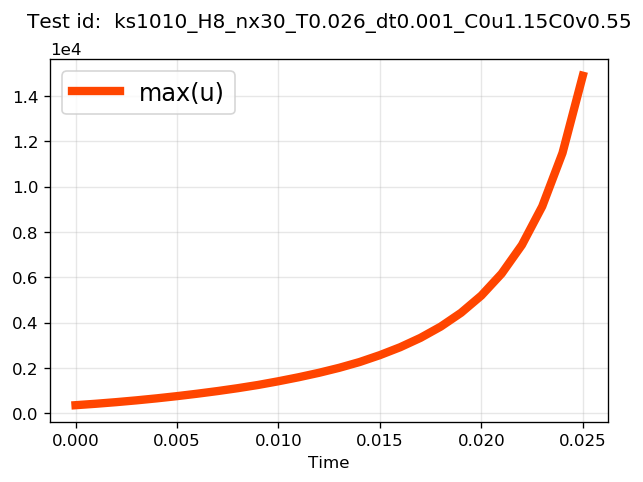
\includegraphics[width=0.48\linewidth]{img/parallel/umax} &
    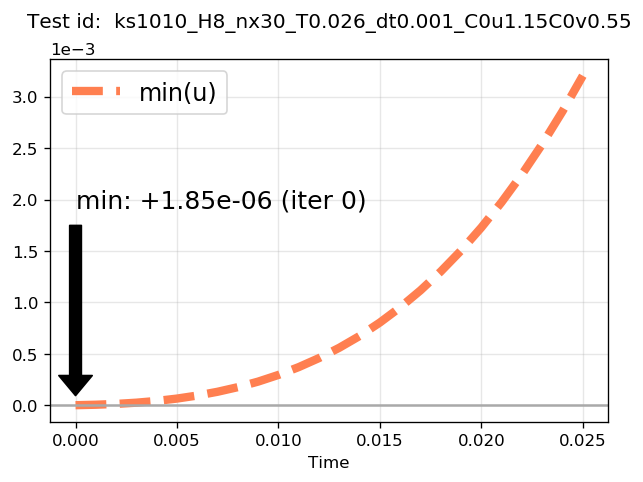
\includegraphics[width=0.48\linewidth]{img/parallel/umin}
    \\
    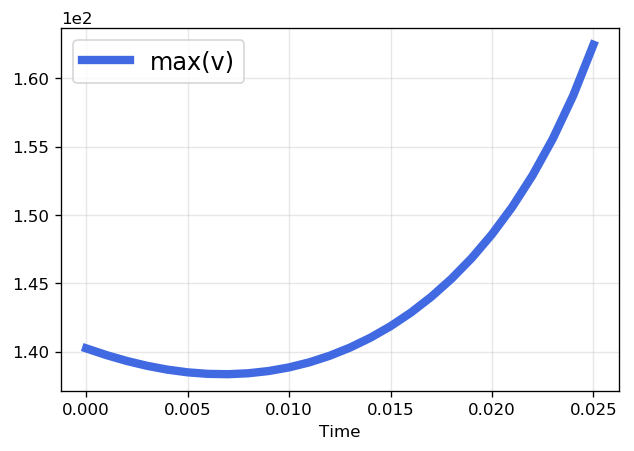
\includegraphics[width=0.48\linewidth]{img/parallel/vmax} &
    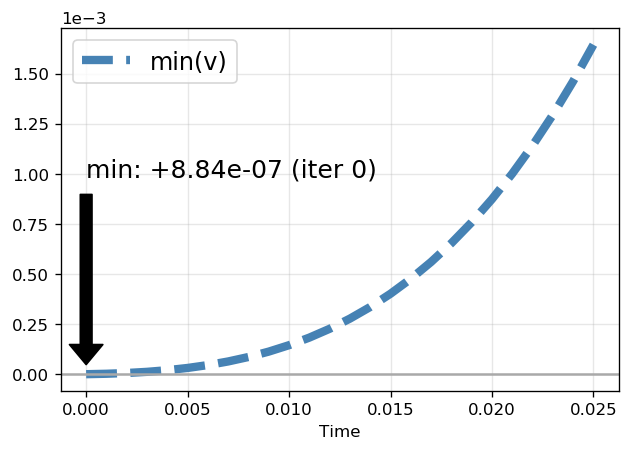
\includegraphics[width=0.48\linewidth]{img/parallel/vmin}
  \end{tabular}
\end{frame}
%=====================================================================

%=====================================================================
\begin{frame}{$P_2$--Bernstein \& Lagrange Polynomials}
%---------------------------------------------------------------------
  ~\vspace*{-2em}
  \begin{flushright}
    \begin{tabular}{@{}m{1em}@{}m{14em}@{}m{14em}@{}}
      & {\scriptsize $P_2$ \textbf{Bernstein} Polynomials}
      & \onslide<2->{\scriptsize $P_2$ \textbf{Lagrange} Polynomials}
      \\ \hline
      \rotatebox[origin=b]{90}{\scriptsize $20\times 20$}
      & 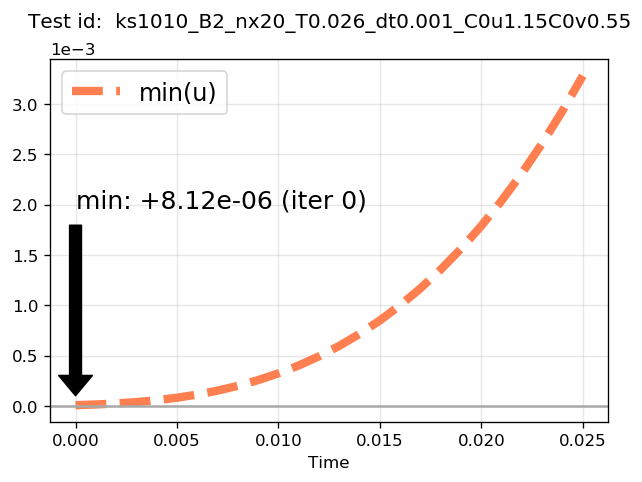
\includegraphics[width=0.9\linewidth]{img/bernstein/umin_B2_nx20}
      & \includegraphics<2->[width=0.9\linewidth]{img/bernstein/umin_L2_nx20}
      \\ %\hline
      \onslide<3>{\rotatebox[origin=c]{90}{\scriptsize $10\times 10$}}
      & \includegraphics<3>[width=0.9\linewidth]{img/bernstein/umin_B2_nx10}
      & \includegraphics<3>[width=0.9\linewidth]{img/bernstein/umin_L2_nx10}
    \end{tabular}
  \end{flushright}
\end{frame}
%=====================================================================

%============================================================================
\section{3D Numerical Tests}
%============================================================================


%=====================================================================
\begin{frame}{Classical Keller-Segel \alert{3D} Numerical Tests}
%---------------------------------------------------------------------
  \begin{itemize}\itemsep1.5em
  \item Now we introduce \alert{3D FE} space \textbf{discretization}
  \item LibMesh makes straightforward the \textbf{jump ``2D $\rightarrow$ 3D''}
  \item \textbf{Computing requirements} are much bigger in the 3D case\\[0.5em]
   \hfill $\Rightarrow$ need of \structure{parallel computing}!
  \item Playing with initial data, \alert{\textbf{3D blow up}} can easily be obtained...
  \end{itemize}
\end{frame}
%=====================================================================

%=====================================================================
\begin{frame}[allowframebreaks]{3D Blow-up in a Sphere}
%---------------------------------------------------------------------
  \foreach \i in {0,...,12} {
    \begin{center}
      \includegraphics[width=0.85\linewidth]{img/blowup3d/blowup3d-\i}%
    \end{center}
    \framebreak
    }
\end{frame}
%=====================================================================


%=====================================================================
\begin{frame}{}
  % ---------------------------------------------------------------------
  \begin{center}
    \large Let us study cases where
    \\[1em]
    \Large \alert{\textbf{\emph{blow-up can be avoided}}} for ``small initial data''
  \end{center}
\end{frame}
%=====================================================================

%=====================================================================
\begin{frame}{Set of Tests}
%---------------------------------------------------------------------
  \begin{itemize}\itemsep1em
  \item $\Omega=\{(x,y,z)\in\mathbb{R}^3:\ x^2+y^2+z^2<4\}$
  \item $(\alpha_0,\alpha_1,\alpha_2,\alpha_3,\alpha_4) = (1,0.2,1,0.1,1)$ (\structure{same parameters than 2D})
  \item $u_0= C_u\*\big(1+\tanh\big(m_u\*(1-x^2-y^2-z^2)\big)\big)$, (\structure{\small$\simeq 0$ outside unit sphere})
    \\[0.2em]
    $v_0= C_v\*\big(1+\tanh\big(m_v\*(1-x^2-y^2-z^2)\big)\big)$ ($m_u$, $m_v$: \structure{initial slope})
  \item $\displaystyle C_u=C_v=k\,\pi$, with $k\in\mathbb{N}$
\item Time discretization: Euler scheme $S=(1,1,1,0)$, $\Tmax=0.3$, $k=0.05$
\item Space discretization: P2-Lagrange, $n_r=4$ refinements from original LibMesh sphere mesh
\end{itemize}
\end{frame}
%=====================================================================

%=====================================================================
\begin{frame}{3D Test 1: $C_u=C_v=\alert{6\,\pi}$: \enspace Blow Up}
%---------------------------------------------------------------------
  \begin{tabular}{cc}
    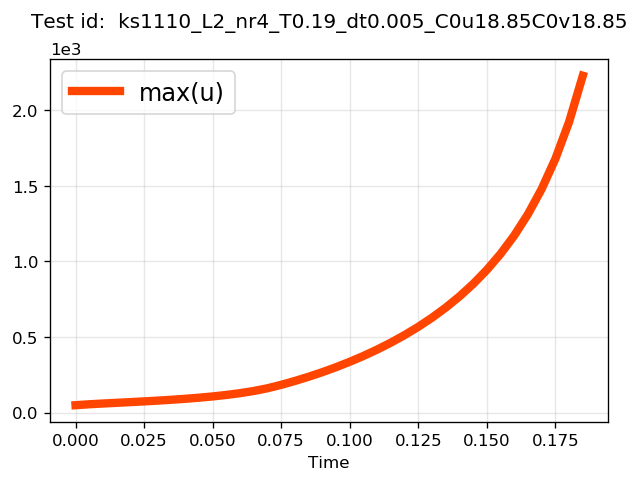
\includegraphics[width=0.48\linewidth]{img/3d/maxu_3d_6pi} &
    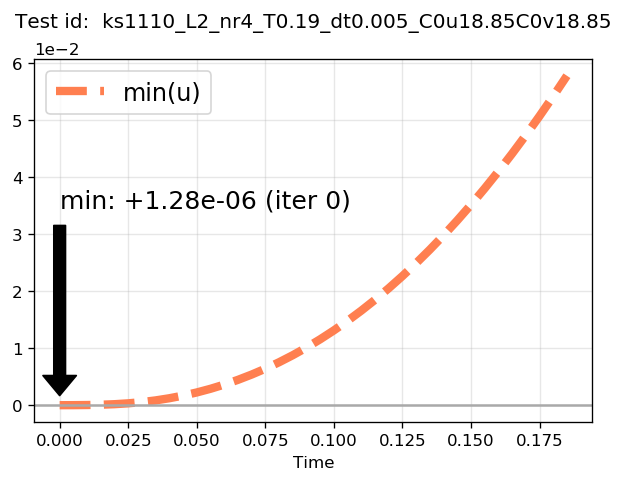
\includegraphics[width=0.48\linewidth]{img/3d/minu_3d_6pi}
    \\
    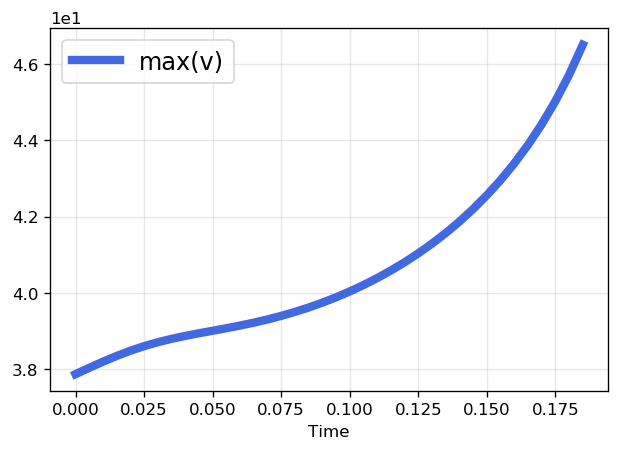
\includegraphics[width=0.48\linewidth]{img/3d/maxv_3d_6pi} &
    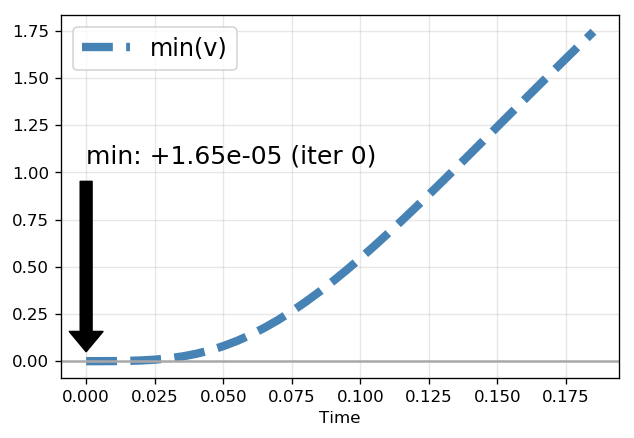
\includegraphics[width=0.48\linewidth]{img/3d/minv_3d_6pi}
  \end{tabular}
\end{frame}
%=====================================================================

%=====================================================================
\begin{frame}{3D Test 2: $C_u=C_v=\alert{5\,\pi}$: \enspace\structure{No Blow Up?}}
%---------------------------------------------------------------------
  \begin{tabular}{cc}
    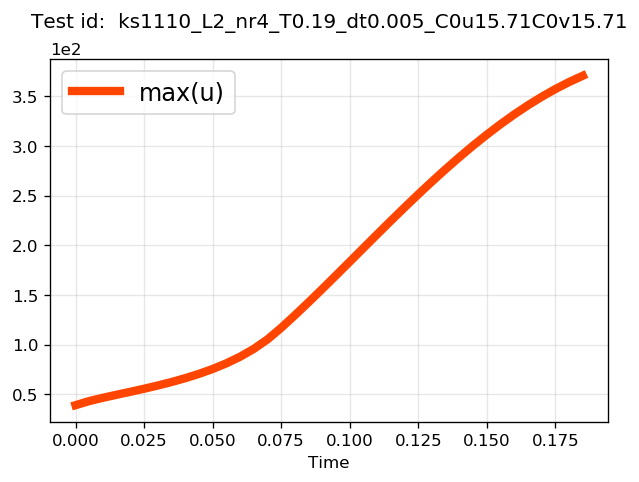
\includegraphics[width=0.48\linewidth]{img/3d/maxu_3d_5pi} &
    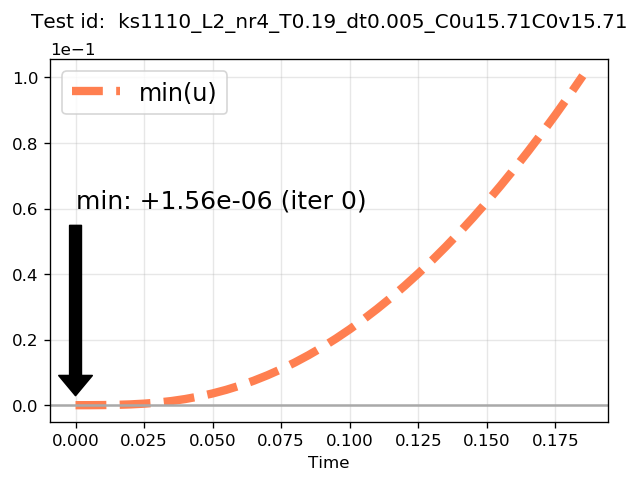
\includegraphics[width=0.48\linewidth]{img/3d/minu_3d_5pi}
    \\
    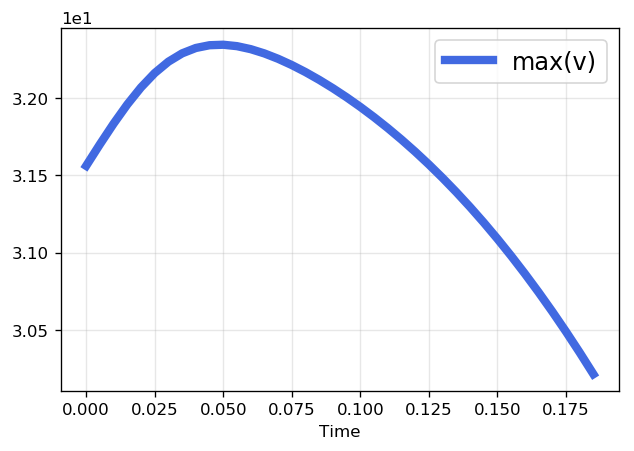
\includegraphics[width=0.48\linewidth]{img/3d/maxv_3d_5pi} &
    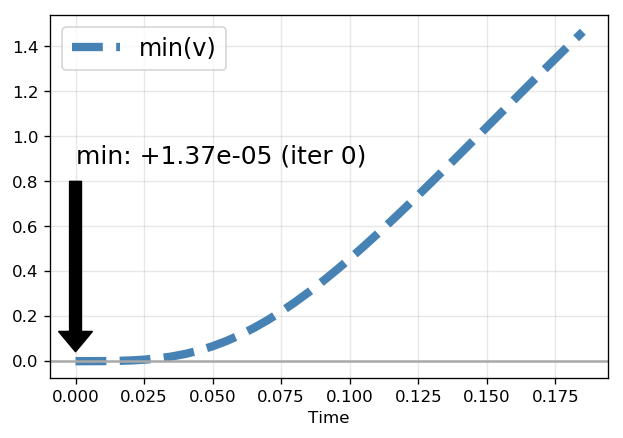
\includegraphics[width=0.48\linewidth]{img/3d/minv_3d_5pi}
  \end{tabular}
\end{frame}
%=====================================================================


%=====================================================================
\begin{frame}{3D Test 3: $C_u=C_v=\alert{4\,\pi}$: \enspace\structure{NO Blow Up!}}
%---------------------------------------------------------------------
  \begin{tabular}{cc}
    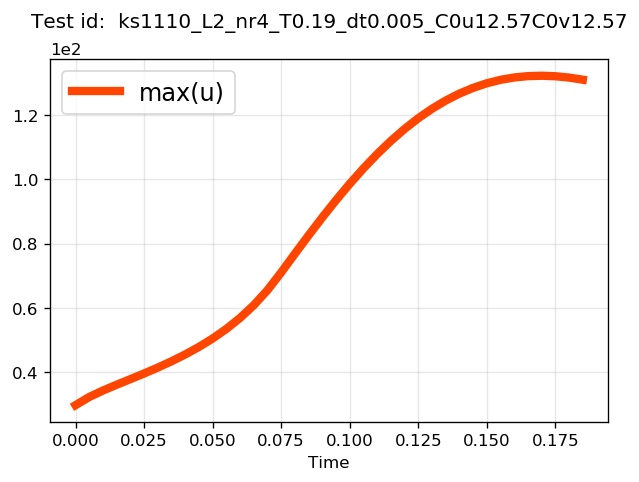
\includegraphics[width=0.48\linewidth]{img/3d/maxu_3d_4pi} &
    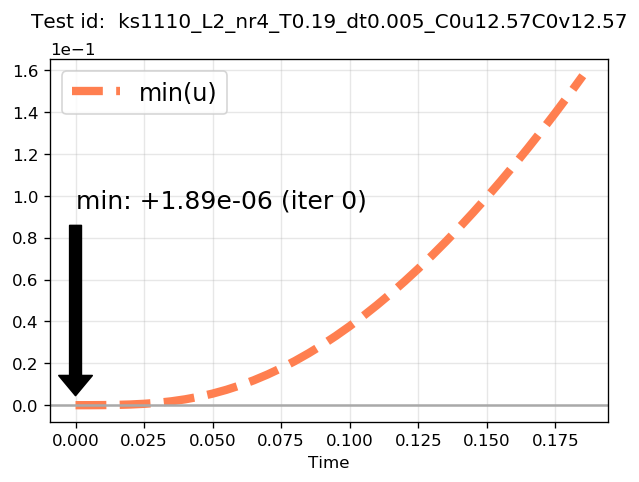
\includegraphics[width=0.48\linewidth]{img/3d/minu_3d_4pi}
    \\
    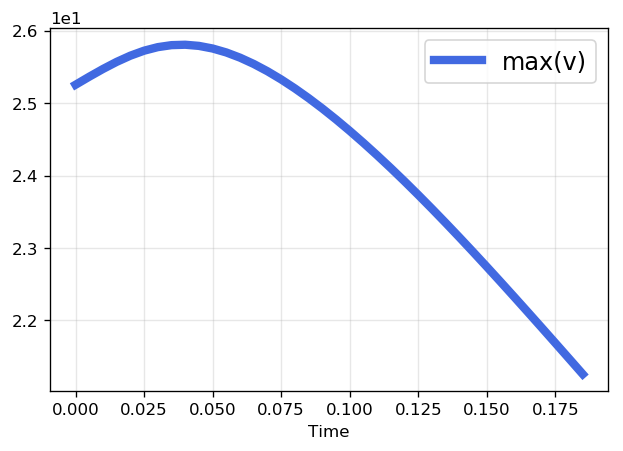
\includegraphics[width=0.48\linewidth]{img/3d/maxv_3d_4pi} &
    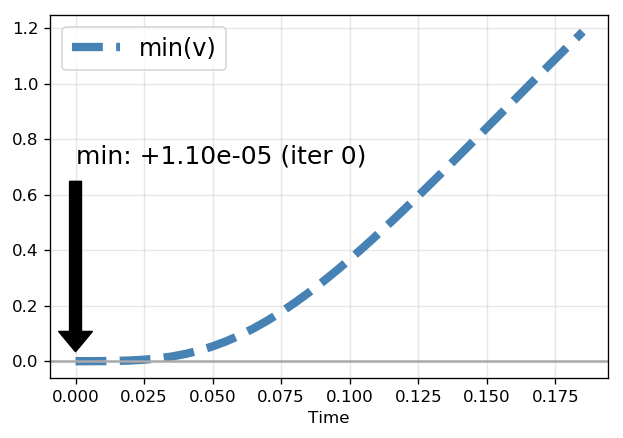
\includegraphics[width=0.48\linewidth]{img/3d/minv_3d_4pi}
  \end{tabular}
\end{frame}
%=====================================================================

%=====================================================================
\begin{frame}[allowframebreaks]{Recent 2D with ideas from 3D initial conditions!}
%---------------------------------------------------------------------
  % \begin{tabular}{cc}
  %   \includegraphics[width=0.48\linewidth]{img/uminus-wave/maxu} &
  %   \includegraphics[width=0.48\linewidth]{img/uminus-wave/minu}
  %   \\
  %   \includegraphics[width=0.48\linewidth]{img/3d/maxv} &
  %   \includegraphics[width=0.48\linewidth]{img/3d/minvi}
  % \end{tabular}
  \foreach \i in {1,5,10,15,20,25,30,35,40,45,50,55,60,65,70,75,80,85,90,85,99} {
    \begin{center}
      \includegraphics[width=0.8\linewidth]{img/uminus-wave/w\i}%
    \end{center}
    \framebreak
    }
\end{frame}

%% ,---------------------------------------------------------------------
%%| Conclusions and future work
%%`---------------------------------------------------------------------
\begin{frame}{Conclussions}
  \begin{itemize}\itemsep0.75em
    \item We \structure{got fun} in classical Keller-Segel numerical simulations
    \item Very interesting problem, in the \textbf{\alert{parabolic/hyperbolic}} edge!
    \item Work for \textbf{future}...
      \begin{itemize}\itemsep0.7em
      \item Numerical approximation of \structure{blow-up}
      \item \structure{Positivity}
      \item Try \alert{DG} and techniques from the hyperbolic world
      \item \structure{Other variants} of Keller-Segel, coupling with fluids...
        \par\smallskip
      \hfill ... and many other things I can't remember now \texttt{:-)}
      \end{itemize}
  \end{itemize}
\end{frame}

\begin{frame}{~}
  \bigskip
  \begin{center}
  \huge ¡Muchas  gracias!
  \vfill~
  \begin{flushright}
    \pgfsetfillopacity{0.4}
    \pgfimage[width=0.9\textwidth]{img/gibraltar-velocity-2d-difumin}
  \end{flushright}
\end{center}
\end{frame}



% %%,-------------
% %%| Bibliography
% %%`-------------

% \setbeamertemplate{footline}[default]

% \begin{frame}[allowframebreaks]{Bibliography}
% \bibliographystyle{alpha}
% %\bibliographystyle{abbrvnat}
% \bibliography{biblio-short.bib}
% \end{frame}
\begin{frame}{Bibliography}
  \bibliographystyle{alpha}
  % \bibliographystyle{plainnat}
  \bibliography{biblio-short}
\end{frame}

\appendix

\begin{frame}{Numeric Dissipation and Source Terms}
  \scriptsize
  \def\arraystretch{2.3} %  1 is the default
  \begin{tabular}{|@{\ }c@{\ }|@{\ \ }c@{\ }|@{\ \ }c@{\ }|}
    \hline
        $(i,\alpha)$  &$N_{i,\alpha}$ & $F_{i,\alpha}$
        \\ \toprule
        $(1,0)$& $0$ & $\displaystyle \frac{k}{2} \int_{\Omega}\left[\left(\frac{\nabla \umm}{\umm}\right)^2\hspace{-0.2cm}+(\nabla\vmm)^2+2\big(\delta_t(\umm)\nabla v_{m+r_2}\big)^2\right]$
        \\ \hline
        $(1,1)$ &0  & 0
        \\ \toprule
        $(2,0)$& 0 & $\frac{k}{2} \displaystyle \int_{\Omega}\left[\left(\frac{u_{m+r_1}}{\umm}\nabla\umm\right)^2\hspace{-0.2cm}+(u_{m+r_1}\nabla\vmm)^2+2\big(\delta_t(\nabla\vmm)\big)^2\right]$
        \\ \hline
        $(2,1)$ &0  & 0
        \\ \toprule
        $(3,0)$& 0 & $\displaystyle \frac{k}{2}\int_{\Omega}\big(\delta_t(\vmm)\big)^2$
        \\ \hline
        $(3,1)$ &$\displaystyle \frac{k}{2}\int_{\Omega}\big(\delta_t(\vmm)\big)^2$ & 0
        \\ \toprule
        $(4,0)$& 0 & 0
        \\\hline
        $(4,1)$ &0  & $\frac{k}{2}\displaystyle\int_{\Omega}\left[\big(\delta_t(\vmm)\big)+\big(\delta_t(\umm)\big)^2\right]$
        \\\bottomrule
      \end{tabular}
\end{frame}

\end{document}


%%% Local Variables:
%%% coding: utf-8
%%% TeX-master: t
%%% mode: latex
%%% ispell-local-dictionary: "english"
%%% End:
